% Chapter 3

\chapter{Programación Matemática} % Main chapter title

\label{Chapter3} % For referencing the chapter elsewhere, use \ref{Chapter1} 
La disciplina que abarca la teoría y la práctica de los métodos de optimización numérica se conoce como programación matemática\cite{antoniou_practical_2007}. El término programación se comienza a utilizar alrededor de 1940 para describir la planificación o programación de actividades dentro de una gran organización. Los programadores encontraron que podían representar la cantidad o el nivel de cada actividad como una variable cuyo valor debía determinarse. Luego podrían describir matemáticamente las restricciones inherentes a la planificación o problema de programación como un conjunto de ecuaciones o desigualdades que involucran las variables. Una solución a todas estas restricciones se consideraba como un plan o programa aceptable. Más tarde, se utilizaría el término matemático
de programación para describir la minimización o maximización de una
función objetivo de varias variables, sujeta a un conjunto de restricciones \cite{takriti1994ampl}. 

Actualmente, la programación matemática es una de las ramas de la investigación de operaciones más desarrolladas y usadas. Las técnicas de programación matemática pueden ser usadas para resolver  problemas de optimización altamente complejos como problemas no lineales de alta dimensionalidad, y multiples restricciones por ejemplo. La teoría matemática en esta área es aplicada tanto para caracterizar puntos óptimos del problema como para proporcionar la base para la mayoría de los algoritmos \cite{nocedal2006numerical}. Por lo tanto en las siguientes secciones se tratan los temas de condiciones de optimalidad de primer y segundo orden para funciones. Luego, se describen los métodos básicos de Programación Matemática identificando sus fortalezas y debilidades.

\section{Información de la Derivada}

El cálculo diferencial es la rama de la matemática que analiza las razones de cambio de cantidades relacionadas, estas pueden considerarse como la pendiente de una tangente a un gráfico de una función. La derivada es el objeto de estudio central del cálculo diferencial donde la idea principal detrás de este concepto es que, en una función $f$ evaluada en un punto $a$, la función $f$ se aproxima a una función lineal en vecindad de $a$. Una definición formal plantea lo siguiente \cite{jean_algebra_2017}:
\begin{defn}

Sea $A$  cualquier subconjunto abierto no vacío de ${\rm I\!R}$ , y $a \in A$. Para cualquier función $f: A \rightarrow {\rm I\!R}$, la derivada de $f$ en $a \in A$ es el límite (si existe):
\begin{equation}
\lim_{h\to 0, \, h \in U} \frac{f(a+h)-f(a)}{h}
\end{equation}
donde $U =\{h \in {\rm I\!R}\,|\, a+h \in A, \, h \neq 0 \}$ este límite se denota como derivada $f'(a)$ o $\frac{\partial f}{\partial x}(a)$. Cuando la derivada existe en todo $a \in A$ se dice que la función es \textit{diferenciable}.
\end{defn}

La derivada de una función $f'$ es otra función, que evaluada en $a$ es la pendiente de la recta tangente a la curva $f$ si esta es representada gráficamente. Este concepto es sumamente importante para la teoría de la programación matemática, ya que una recta horizontal tangente a un punto de $f$ describe un cambio de comportamiento en la función. Estos puntos cuyas rectas tangentes son horizontales se denominan \textit{puntos estacionarios} y pueden satisfacer la condición de óptimo de la función. Esto no siempre se cumple ya que puede tratarse de un punto de inflexión. Luego, el cálculo de los puntos estacionarios de la función consiste en hallar aquellos cuya recta tangente tenga pendiente igual cero, esto es $f'(x)=0$.Véase figura . Este procedimiento se conoce como la \textit{prueba de la primera derivada}.

\begin{figure}
\centering
  \begin{tikzpicture}[scale=1]


     \draw [->] (-1,0) -- (11,0) node [right] {$x$};
     \draw [->] (0,-1) -- (0,6) node [above] {$y$};
     \node at (0,0) [below left] {$0$};
     \draw  plot[smooth, tension=.8] coordinates{(1,-0.5) (2.5,3) (5,1.5)  (7.8,4) (10,-1)};
     \node at (0.8,-0.25) {$a$};
     \node at (9.5,-0.25) {$b$};
     \draw[dashed] (2.7,3.05) -- (2.7,0);
     \draw[dashed] (4.9,1.5) -- (4.9,0);
     \draw[dashed] (7.52,4.05) -- (7.52,0);
     
     \node at (2.7,-0.25) {$x_{1}$};
     \node at (4.9,-0.25) {$x_{2}$};
     \node at (7.5,-0.25) {$x_{3}$};
     \draw (2,3.05) -- (4,3.05);
     \draw (4,1.5) -- (6,1.5);
     \draw (6.5,4.05) -- (8.25,4.05);
     \node at (2.7,3.5) {\small $f'(x_{1})=0$};
     \node at (4.9,2.2) {\small $f'(x_{2})=0$};
     \node at (7.3,4.5) {\small $f'(x_{3})=0$};
     \node at (9.5,2.5) {\small $f(x)$};
\end{tikzpicture}
\caption{Puntos estacionarios y sus rectas tangentes}
\end{figure}

Los puntos estacionarios pueden ser mínimos, máximos o puntos de inflexión. Para diferenciar los puntos es necesario utilizar información de la segunda derivada.  La segunda derivada de la función indica el cambio en la pendiente. Una función con $f''(x)> 0$ es convexa en $x$. O sea, la función se curva hacia arriba a medida que aumenta la pendiente. Por otra parte, una función con pendiente decreciente, $f'' (x) <0$ es cóncava hacia abajo en $x$. La \textit{prueba de la segunda derivada} es capaz de diferenciar mínimos y máximos de la siguiente forma:
\\
\\
\begin{defn}
Dada una función diferenciable $f:A \to {\rm I\!R}$  y un punto $x \in A$ se cumple que:
\begin{enumerate}
\item Si $ \frac{\partial f}{\partial x} =0$ y $\frac{\partial^2 f}{\partial^2 x} >0$, el punto $x$ es un mínimo.
\item Si $ \frac{\partial f}{\partial x} =0$ y  $\frac{\partial^2 f}{\partial^2 x} <0$, el punto $x$ es un máximo.
\end{enumerate}
\end{defn}

A la izquierda de un mínimo, la función decrece. A la derecha la curva se eleva. La pendiente ha cambiado de negativa a positiva. El gráfico se dobla hacia arriba y $f''(x)> 0$. Por el contrario a la derecha del máximo, la pendiente pasa de positiva a negativa en la vecindad del mínimo. En el caso excepcional,
cuando $f'(x) = 0$ y también $f''(x) = 0$ la regla no se cumple y el punto puede ser cualquiera de los tres tipos de puntos estacionarios. Se debe señalar que la información de $f'(x)$ y $f''(x)$ es sólo  local. Para encontrar un mínimo o máximo global, se necesita información sobre todo dominio. Además se asume que la función es continua y diferenciable en todo su dominio, lo cual no siempre se satisface \cite{gilbert_calculus_2010}.
\section{Información del Gradiente}
Los métodos descritos en la sección anterior solo pueden ser aplicados para funciones univariables. Para analizar el comportamiento de funciones de más de una variable se utiliza la información del gradiente de la función. Si una función multivariable $f(\vec{x})$, tiene una derivada continua de primer orden $f'(\vec{x})$ el gradiente de $f(\vec{x})$ se define como un vector compuesto por las derivadas parciales de la función objetivo:
\begin{equation}
\nabla f(\vec{x})=\bigg[ \frac{\partial f}{\partial x_1}, \frac{\partial f}{\partial x_2},\ldots,\frac{\partial f}{\partial x_n}\bigg]^T
\end{equation}

La derivada parcial  $\frac{\partial f}{\partial x_i}$ con $i=\{1,2,\ldots,n\}$ trata las restantes $n-1$ variables como constante y viceversa. Cada derivada parcial $\frac{\partial f}{\partial x_i}$ evaluada en un punto cualquiera denota la pendiente en la dirección $x_i$. Si se concibe la función como una hiper-superficie, el gradiente describe en qué dirección la superficie toma un valor máximo. Por tanto indica la dirección de ascenso, y su magnitud $|\nabla f(\vec{x})|$ indica el grado de inclinación de la superficie \cite{gilbert_calculus_2010}. La Figura \ref{fig: gradiente} muestra a la izquierda el capo vectorial de la superficie $x e^{(-x^2-y^2)}$. Se puede observar cómo la dirección del gradiente indica hacia donde la superficie asciende y su longitud es mayor en áreas con cambios de ascenso máximo. Luego en los puntos donde la función se hace plana, o llega a su valor máximo o mínimo, el gradiente tiende a desaparecer.  


\begin{figure}[h]  
\centering 
\begin{subfigure}[b]{0.49\linewidth}

\begin{tikzpicture}[scale=0.8]
    \begin{axis}[
        domain=-2:2,
        view={0}{90},
        axis background/.style={fill=white},
    ]
        \addplot3[contour gnuplot={number=9,
            labels=false},thick]
                {exp(0-x*x-y*y)*x};
        \addplot3[blue,
            quiver={
             u={exp(0-x*x-y*y)*(1-2*x*x)},
             v={exp(0-x*x-y*y)*(-2*x*y)},
             scale arrows=0.3,
            },
            -stealth,samples=15]
                {exp(0-x*x-y*y)*x};
    \end{axis}
\end{tikzpicture}
 \caption{Campo vectorial} \label{fig:M1} 
\end{subfigure}
\begin{subfigure}[b]{0.49\linewidth}
  
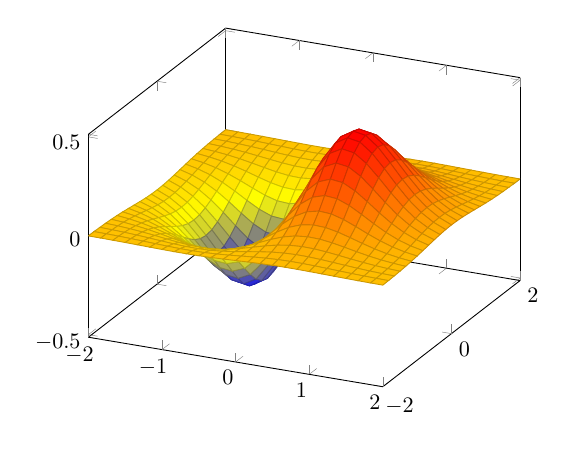
\begin{tikzpicture}[scale=0.8]
  \begin{axis}[domain=-2:2,y domain=-2:2]
    \addplot3[surf] {exp(0-x*x-y*y)*x};
  \end{axis}
\end{tikzpicture}
 \caption{Superficie} \label{fig:M1} 

\end{subfigure}
 \caption{Función $x  \exp(-x^2-y^2)$ } \label{fig: gradiente} 

\end{figure}

De lo planteado en la sección anterior se entiende que las derivadas parciales tomarán valores de cero para los puntos estacionarios de la función. Luego, el cálculo de los puntos estacionarios para una función multivariable consiste en resolver el siguiente sistema de  ecuaciones \cite{soliman_mathematical_2012}:
\begin{center}
\begin{equation}
 \frac{\partial f}{\partial x_1}=0
\end{equation}
\begin{equation}
 \frac{\partial f}{\partial x_2}=0
\end{equation}
\vdots
\begin{equation}
 \frac{\partial f}{\partial x_n}=0
\end{equation}
\end{center}

Las ecuaciones 3.3, 3.4 y 3.5 representan un sistema de $n$ ecuaciones con $n$ incógnitas. Luego, para determinar determinar cuáles de los puntos estacionarios son mínimos o máximos se utiliza la información proporcionada por la matriz Hessiana. La matriz Hessiana representa la segunda derivada de una función de más de una variable. Si la función $f$ tiene segundas derivadas parciales, entonces la matriz de Hessiana se define como:
\begin{equation}
 H(\vec{x})=
 \begin{bmatrix}
    \frac{\partial^2 f}{\partial^2 x_1} & \frac{\partial^2 f}{\partial x_1 \partial x_2} & \dots  & \frac{\partial^2 f}{\partial x_1 \partial x_n} \\
    \frac{\partial^2 f}{\partial x_2 \partial x_1} & \frac{\partial^2 f}{\partial^2 x_2} & \dots  & \frac{\partial^2 f}{\partial x_2 \partial x_n}\\
    \vdots & \vdots & \ddots & \vdots \\
    \frac{\partial^2 f}{\partial x_n \partial x_1} & \frac{\partial^2 f}{\partial x_n \partial x_2} & \dots  & \frac{\partial^2 f}{\partial^2 x_n }
\end{bmatrix}
 \end{equation}

Si la matriz $H(\vec{x})$ es positiva definida, esto es, que su determinante sea mayor que cero; entonces $\vec{x}$ representa un mínimo de la función $f$, en cambio si la matriz $H(\vec{x})$ es definida negativa, entonces $f(\vec{x})$ es un máximo \cite{antoniou_practical_2007}. En próximas secciones se describe cómo la matriz Hessiana no solo puede ser utilizada para determinar condiciones de optimalidad, sino que también se utiliza para calcular direcciones de búsqueda en métodos basados en gradiente.

\section{Métodos de Optimización Univariable}
A pesar de que problemas no restringidos, con función objetivo de una sola variable son poco comunes en situaciones prácticas, la determinación del mínimo de una función de valor real univariable, desempeña un rol activo en la optimización no lineal. Los métodos univariables son importantes primeramente desde el punto de vista teórico y demostrativo. Además, como se verá en la sección 3.4, este tipo de procedimientos de minimización se pueden aplicar varias veces en un problema multivariable. En efecto, los algoritmos de optimización univarible forman parte de los bloques básicos de operación de los algoritmos de optimización multivariables.  Estos métodos se clasifican de forma general en algoritmos basados en gradiente y no basados en gradiente. En las siguientes secciones se discuten algunos de los más populares. Los dos primeros métodos son la Búsqueda de Fibonacci y el método de la Sección Dorada, los cuales entran en la clasificación de los no basados en gradiente y además son métodos de eliminación de regiones bien conocidos. Por último se presenta el método de Newton-Rapson, el cual utiliza información de la primera y la segunda derivada para encontrar la dirección óptima de búsqueda. 

\subsection{Método de Fibonacci }
El método de Fibonacci se considera como un método de eliminación de regiones pues reduce el intervalo de búsqueda de acuerdo a la serie de Fibonacci definida por la recursión $F_k = F_{k-1} + F_{k-2}$.  Esta expresión genera la secuencia, $F_i= \{1,\, 1,\, 2, 3,\, 5,\, 8,\, 13,\, ...,\,F\} = \{F_0,\, F_1,\, F_2,\, F_3,\, F_4,\, F_5,\, F_6,\, ...\,,\,F_n \}$, conocida como secuencia de Fibonacci que se produce en varias ramas de las matemáticas. Este método realiza una serie de iteraciones acotando el intervalo de acuerdo a la siguiente razón:
\begin{equation}
 I_n = \frac{I_0}{ F_n}
 \end{equation}
Esto es, que para la iteración $n$ el tamaño del intervalo original será reducido al $n$-ésimo número de Fibonacci. La secuencia de intervalos de Fibonacci sólo se puede generar si se conoce $n$. Luego, si el objetivo de la optimización es encontrar $x^*$ dentro de una tolerancia prescrita, el $n$ requerido se puede deducir fácilmente usando Ecuación 3.7. Los métodos de eliminación de regiones asumen que $f(x)$ es estrictamente unimodal en $I$, donde siempre se divide el intervalo actual en dos regiones; el intervalo que contenga un punto con menor valor de la función objetivo será elegido y se convierte en el intervalo actual. Por tanto, se conoce que $n$ será menor si el mínimo de $f(x)$ es poco profundo y alto si $f(x)$ varía rápidamente en la vecindad de la solución. 
\begin{figure}
\centering
\begin{tikzpicture}
\begin{axis}[width=5in,axis equal image,
    axis lines=middle,
    xmin=0,xmax=8,
    xlabel=$x$,ylabel=$y$,
    ymin=-1.4,ymax=4,
    xtick={\empty},ytick={\empty}, axis on top
]

% 
%\addplot[thick,domain=0.25:7,black,name path = A]  {-x/3 + 2.75} coordinate[pos=0.4] (m) ;
\draw[thick,black, name path =B] (0.15,4) .. controls (1,1.5) and (5,0) .. (7,1.5) node[pos=0.95, color=black, right]  {$f(x)$} coordinate[pos=0.075] (a1)  coordinate[pos=0.95] (a2) coordinate[pos=0.7] (m) coordinate[pos=0.43] (a)
coordinate[pos=0.63] (b);
%\path [name intersections={of=A and B, by={a,b}}];

% 
\draw[densely dashed, name path=A] (0,0) -| node[pos=0.5, color=black, label=below:$a$] {}(a1);
\draw[densely dashed, name path=E] (0,0) -| node[pos=0.5, color=black, label=below:$x_{ak}$] {}(a);
\draw[densely dashed, name path=D] (4,0) -|node[pos=0.5, color=black, label=below:$x^*$] {} (m);
\draw[densely dashed, name path=L] (0,0) -|node[pos=0.5, color=black, label=below:$x_{bk}$] {}(b);
\draw[densely dashed, name path=F] (0,0) -|node[pos=0.5, color=black, label=below:$b$] {}(a2);

\draw[arrows=<->] (0.35,-0.6)-- node[below] {$I_{k+1}$} (4.2,-0.6);
\draw[arrows=<->] (4.2,-0.6)   -- node[below]{$I_{k+2}$} (6.7,-0.6);
\draw[arrows=<->] (0.35,-1.3)   -- node[below]{$I_k$} (6.7,-1.3);

% 
\path [name intersections={of=B and D, by={c}}] node[fill,circle,inner sep=1pt] at (c) {}; 
\path [name intersections={of=B and A, by={c1}}] node[fill,circle,inner sep=1pt] at (c1) {}; 
\path [name intersections={of=B and E, by={c2}}] node[fill,circle,inner sep=1pt,label=right:$f(x_1)$] at (c2) {}; 
\path [name intersections={of=B and L, by={c3}}] node[fill,circle,inner sep=1pt,label=above:$f(x_2)$] at (c3) {}; 
\path [name intersections={of=B and F, by={c4}}] node[fill,circle,inner sep=1pt] at (c4) {}; 
% 
%\node[anchor=south west, text=black] (d) at (0.75,3) {$f[\alpha x_{1}+(1-\alpha)x_{2}]$};
%\node[anchor=south west, text=black] (e) at (5,2.5) {$\alpha f(x_{1})+(1-\alpha)f(x_{2})$};
%\draw[-{Latex[width=4pt,length=6pt]}, densely dashed] (d) -- (c);
%\draw[-{Latex[width=4pt,length=6pt]}, densely dashed] (e) -- (m);
\end{axis}
\end{tikzpicture}
\caption{Reducción de intervalos en el método de Fibonacci.}

\end{figure}

Los principios anteriores se pueden usar para implementar el método. Se comienza definiendo un intervalo $I_0$ y los  límites iniciales inferior y superior $x_{L\,0}$ y $x_{U\,0}$ respectivamente. Donde $x_{a\,0}$ y  $x_{b\,0}$ son dos puntos interiores en el intervalo $I_k$. Además, se conoce el valor de $n$, y la descripción matemática de $f(x)$. En cada iteración se calculan intervalos sucesivos, se evalúa $f(x)$, se actualiza y selecciona el intervalo correspondiente. En la k-ésima iteración, los valores de  $x_{L\,k}$, $x_{U\,k}$, $x_{a\,k}$, $x_{b\,k}$, $f(x_{a\,k})$,  $f(x_{b\,k})$ y el intervalo $I_{k + 1}$ son conocidos. Luego, el valor de $I_{k + 2}$ se calcula mediante la siguiente expresión:
\begin{equation}
 I_{k+2} = \frac{F_{n-k-1}}{ F_{n-k}}I_{k+1}
 \end{equation}
La actualización de los puntos interiores y los intervalos se realiza atendiendo las siguientes condiciones:
\begin{enumerate}
\item Si $f(x_{a\,k}) > f(x_{b\,k})$ entonces $x^*$ está en el intervalo $[ x_{a\,k}, x_{U\,k}]$ por tanto $ x_{L\,k+1} =x_{L\,k}$ y $ x_{U\,k+1} =x_{b\,k}$  son los nuevos límites del intervalo  $I_{k + 1}$. Luego, los puntos interiores de este intervalo serían $x_{a\,k+1} =x_{b\,k}$ y  $x_{b\,k+1} =x_{L\,k+1}+I_{k+2}$.

\item Si $f(x_{a\,k}) < f(x_{b\,k})$ entonces $x^*$ está en el intervalo $[x_{L\,k}, x_{b\,k}]$ por tanto $ x_{L\,k+1} =x_{a\,k}$ y $ x_{U\,k+1} =x_{U\,k}$. Los puntos interiores de este intervalo toman entonces los siguientes valores $x_{a\,k+1} =x_{U\,k+1}-I_{k+2}$ y  $x_{b\,k+1} =x_{a\,k}$.
\end{enumerate}

Aunque es poco probable, se puede dar el caso en que $f(x_{a\,k}) = f(x_{b\,k})$. Entonces se pueden aplicar cualquiera de las asignaciones anteriores ya que $x^*$ está contenido en ambos intervalos  $[x_{L\,k}, x_{b\,k}]$ y  $[ x_{a\,k}, x_{U\,k}]$. Este procedimiento se repite hasta que $k = n - 2$ en cuyo caso $I_k + 2 = I_n$ y $x^* = x_{a\,k+1} =  x_{b\,k+1}$ \cite{antoniou_practical_2007}.

\subsection{Método de la Sección Dorada}
Este método tiene sus antecedentes en la antigua Grecia donde los arquitectos griegos afirmaban que un edificio con lados $d$ y $b$ satisficiera la siguiente relación tendría mejores propiedades:
\begin{center}
\begin{equation}
\frac{d+b}{d}=\frac{d}{b}= \phi=1.618034
\end{equation}
\end{center}

La proporción descrita por la ecuación anterior se denomina razón dorada. En este método, como en la búsqueda de Fibonacci, se genera una secuencia de intervalos $\{I_1, I_2, I_3, ...\}$ utilizando la razón dorada. Sin embargo, a diferencia del método de Fibonacci, no es necesario especificar el número total de iteraciones como parámetro de inicio. La regla según la cual se generan las longitudes de los intervalos sucesivos es que la relación de dos intervalos adyacentes debe ser constante igual a $\phi$, es decir:
\begin{equation}
\begin{aligned}
 I_1 = I_2 + I_3 & &\\
 I_2 = I_3 + I_4 & &\\
 \vdots & &
\\
\frac{I_2}{I_{1}}=\frac{I_3}{I_{3}}= \frac{I_4}{I_{3}}=\ldots=\phi
\end{aligned}
\end{equation}
Si toma la primera ecuación a conveniencia y se sustituye $I_2 =  \phi I_1 $ y  $I_3 = \phi I_2=\phi^2 I_1$ se obtiene la ecuación:
\begin{equation}
 \phi^2 + \phi -1=0
\end{equation}
Cuyas raíces son $\phi=\frac{1 \pm \sqrt[]{5}}{2}$. 
La estrategia de reducción de intervalo en el algoritmo de sección dorada sigue los pasos utilizados en el algoritmo de Fibonacci, excepto que la Ecuación 3.8 se reemplaza $\frac{F_{n-k-1}}{ F_{n-k}}$ por la razón áurea $\phi=\frac{1 - \sqrt[]{5}}{2}$. El método de sección dorada es un método robusto que se puede integrar de manera eficiente con otros métodos de búsqueda multivariable \cite{belegundu_optimization_2011}.
%%%%
\subsection{Método de Newton-Rapson}
El método fue diseñado por Joseph Raphson en 1960, basándose en los métodos de Isaac Newton para evaluar la raíz de una ecuación usando una secuencia de polinomios.  El método de Newton-Raphson es una técnica de búsqueda de raíz en la que se evalúa la ecuación $f'(x) = 0$. Usando la serie de Taylor, la función $f'(x)$ se puede aproximar como:
\begin{equation}
 f'(x_k) + f''(x_k)\Delta x
\end{equation}
Donde $\Delta x=  x_{k+1}-x_k$. Haciendo la ecuación anterior igual a cero, el siguiente punto de aproximación puede darse como:
\begin{equation}
 x_{k+1}=x_k - \frac{f'(x_k)}{f''(x_k)} 
\end{equation}
El procedimiento realizado por el método es iterativo comenzando por un punto $x_0$. Luego en la k-ésima iteración se mejora de acuerdo a la ecuación anterior, hasta que la diferencia entre $x_k$  y $x_{k-1}$ sea menor que un tolarancia $\epsilon$. Al igual que la mayoría de los métodos de programación matemática, la convergencia del método de Newton-Raphson es sensible al punto inicial. Además, de que la convergencia se ralentiza cuando el valor de la derivada es cercano a cero, en este método se asume que la segunda derivada de la función existe lo cual puede limitar su aplicación \cite{rao_engineering_2009}.
\section{Métodos de optimización multivariable}

Las técnicas de solución para problemas de optimización multivariable y sin restricciones se pueden agrupar en métodos basados en gradiente y métodos directos de búsqueda. Los métodos basados en gradientes requieren información de la derivada de la función para constituir direcciones de búsqueda hacia el mínimo. En los métodos directos, la solución se obtiene utilizando únicamente evaluaciones de la función objetivo. El enfoque general es explorar el espacio de búsqueda mediante una estrategia sistemática con el fin de encontrar una trayectoria que conduzca progresivamente a valores reducidos de la función objetivo. Los métodos de búsqueda multidimensionales pueden ser considerados como análogos a sus contrapartes unidimensionales, y al igual que estos últimos, presentan deficiencias similares en cada grupo.  

Los métodos de gradiente se pueden agrupar en dos clases, métodos de primer orden y segundo orden. Los métodos de primer orden se basan en la aproximación lineal de la serie de Taylor y, por lo tanto, implican sólo el gradiente de la función. Los métodos de segundo orden, por otro lado, se basan en la aproximación cuadrática de las series de Taylor por lo que utilizan además información de la matriz Hessiana. La información del gradiente, la matriz Hessiana o la combinación de ambos, permite encontrar una dirección de búsqueda donde la función tienen su mayor inclinación de descenso. Una vez que se identifica la dirección de búsqueda, se necesita evaluar cuánto se debe mover el punto actual en esa dirección para minimizar la función. Este es un problema unidimensional en cual se puede aplicar cualquiera de los métodos de optimización univariable descritos en las secciones anteriores  \cite{luenberger_linear_2015}.

Los métodos directos no requieren información de la primera derivadas o  segunda derivada para encontrar la dirección de búsqueda. En su lugar, ésta se determina mediante las evaluaciones de función, así como por las direcciones de búsqueda calculadas a partir de iteraciones anteriores. Esta característica, permite que este tipo de métodos puedan ser aplicados a un espectro más amplio de problemas de optimización \cite{belegundu_optimization_2011}. En las secciones correspondientes, los algoritmos de los métodos directos serán descritos con mayor detalle, debido a que,  por sus características son los principales candidatos para la hirbidación con operadores de algoritmos evolutivos. 

\subsection{Método del Descenso Inclinado}
El funcionamiento básico de  la mayoría de las técnicas de optimización basadas en gradiente, consiste en encontrar la tasa de cambio de una función objetivo con respecto a un parámetro $\lambda$ a lo largo de una dirección determinada, $S_k$, que se aleja de un punto $\vec{x}_k$. Cualquier punto en la dirección $S_k$ se puede expresar $\vec{x}_k=\vec{x}_k+ \lambda S_k$. Si el objetivo es la minimización, entonces la tarea consiste en encontrar la tasa de cambio respecto a $\lambda$ en la dirección $S_i$ que minimice la función objetivo. Si se conoce que el gradiente de una función $\nabla f(x)$ indica la dirección de ascenso, y su magnitud $|\nabla f(\vec{x})|$ el grado de inclinación de la función en esa dirección; el negativo del gradiente nos indica dirección hacia donde existe mayor descenso de la función. 

La utilización del negativo del vector de gradiente como una dirección para la minimización fue realizado por primera vez por Cauchy en 1847. En este método, también conocido como método de Cauchy, se comienza desde un punto inicial $\vec{x}_0$ y se avanzamos iterativamente a lo largo de las direcciones de descenso cada vez más inclinadas hasta encontrar el punto óptimo. El método de descenso más inclinado se puede resumir en los siguientes pasos \cite{rao_engineering_2009}:
\begin{enumerate}
\item Definir un punto inicial arbitrario $\vec{x}_0$ y número de iteración $k =0$
\item Calcular la dirección de búsqueda $S_k = -\nabla f(\vec{x}_k)$
\item Determinar la longitud óptima del paso $\lambda^*_k$ en la dirección $S_k$ que minimice la función objetivo en el punto:
\begin{equation}
\vec{x}_{k+1} = \vec{x}_k +\lambda^*_k S_k
\end{equation}
Esto es,
\begin{equation}
\vec{x}_{k+1} = \vec{x}_k -\nabla f(\vec{x}_k)\lambda^*_k
\end{equation}
\item Probar optimalidad del nuevo $\vec{x}_{k+1}$. Si $\vec{x}_{k+1} $ es óptimo, terminar el proceso. De lo contrario, ir al paso 5.
\item Actualizar el número de iteración $k = k +1$ e ir al paso 2.
\end{enumerate}

El método de descenso inclinado es el método más representativo de los basados en gradiente. Es importante destacar que para hallar $\lambda^*_k$ se debe minimizar la función que describe la ecuación 3.15, conocidos $x_i$ y el vector gradiente evaluado en este punto. En este caso se puede aplicar cualquiera de los métodos de búsqueda unidimensional. Si bien es cierto que búsqueda unidimensional comienza en la mejor dirección, la dirección de descenso más pronunciado es una propiedad local, por tanto el método no es realmente efectivo en la mayoría de los problemas con funciones multimodales.
\subsection{Método de Newton}
El método de Newton se comporta de manera similar al de Cauchy. Sin embargo, utiliza las segundas derivadas o la matriz de Hessiana de la función objetivo para calcular la dirección de búsqueda. Este método, cuando converge, lo hace a un ritmo más rápido que los métodos de primer orden como el método de Cauchy. La idea fundamental aquí, es construir una aproximación cuadrática a la función $f (x)$ y realizar su minimización. Por lo tanto, en un punto $x_k$, se construye la aproximación cuadrática de la función \cite{belegundu_optimization_2011}:
\begin{equation}
q(\vec{x})= f(\vec{x}_k) +\nabla f(\vec{x}_k)^T (\vec{x}-\vec{x}_k) +\frac{1}{2} (\vec{x}-\textbf{x}_k)^T \nabla^2 f(\vec{x}) (\vec{x}-\vec{x}_k)
\end{equation}
El mínimo de esta ecuación se encuentra en $ \nabla q(\vec{x})=0$, asumiendo que  $\nabla^2 f(\vec{x})$ es positiva y definida, y denotamos $S_k=(\vec{x}-\vec{x}_k)$  tenemos que:
\begin{equation}
  \big[ \nabla^2 f(\vec{x}) \big ] S_k=- \nabla f(\vec{x}) 
\end{equation}
Despejando  $\big[ \nabla^2 f(\vec{x}) \big ]$ de la ecuación anterior se obtiene la dirección de búsqueda:
\begin{equation}
S_k=- \nabla f(\vec{x})   \big[ \nabla^2 f(\vec{x}) \big ]^{-1}
\end{equation}

Nótese que $ \big[ \nabla^2 f(\vec{x}) \big ]$  es la matriz Hessiana $H(\vec{x})$ de $f$ y $\big[ \nabla^2 f(\vec{x}) \big ]^{-1}$ su inversa. A partir de este punto, el método se comporta de forma similar al de Cauchy, generando una secuencia de puntos $\vec{x}_k$ en direcciones descendentes $S_k$. El punto límite de esta secuencia es el óptimo $\vec{x}^*$ donde $\nabla f(\vec{x}^*) = 0$. 

De la ecuación 3.16, se deriva que si la función es cuadrática con una matriz Hessiana definida, entonces el método de Newton logrará converger en la primera iteración. Sin embargo, para funciones no cuadráticas el método de Newton no converge a menos que el punto de partida sea cercano al óptimo. Si la función presenta cambios de modalidad frecuentes en su dominio, una aproximación cuadrática puede resultar inefectiva. 

Por otra parte, las condiciones de suficiencia que requieren que $H (\vec{x}^*)$ sea positiva definida en $\vec{x}^*$ no imponen restricciones a la $H$ durante el proceso iterativo en un punto $\vec{x}_k$.  Entonces, si  $H (\vec{x}_k)$ no es positivo o si es singular, entonces $q (\vec{x})$ puede no tener un mínimo. La ecuación (3.17) puede no resolverse, o si puede resolverse, puede empeorar punto que el punto actual. Por supuesto, si $f$ es estrictamente convexa, entonces su Hessiana es definitivamente definida y el método de Newton puede aplicarse de manera efectiva \cite{belegundu_optimization_2011}.
\subsection{Método Nelder-Mead}\label{sec: Metodo NM}
Basándose  en el trabajo de Spendley \cite{spendley_sequential_1962} donde se plantea una técnica para el seguimiento de condiciones operativas óptimas, mediante la evaluación de la salida de un sistema en un conjunto de puntos que forman un simplex en el espacio, Nelder y Mead propusieron un algoritmo que realiza la minimización de una función en un espacio de $n$ variables mediante operaciones sobre un simplex que se adapta al  ``paisaje local'', alargándose por largos planos inclinados, cambiando de dirección al encontrar un valle en un ángulo determinado y contrayéndose en la vecindad de un mínimo. El algoritmo original fue diseñado para optimización sin restricciones \cite{nelder_simplex_1965}.
\begin{algorithm}
	\begin{algorithmic}[1]
		\STATE Elegir parámetros: $\beta>0, \gamma \in (0,1)$ y un parámetro de finalización $\epsilon$. 
		\STATE Generar un simplex inicial.
		\label{lin:lineaRara}
		\WHILE {$  \epsilon  \leq \big\{ \sum_{i=1}^{N+1} \frac{((x_i)-f(xc))^2}{N+1} \big\}^\frac{1}{2}$}
		\STATE Elegir $\vec{x}_h$ (peor punto), $\vec{x}_l$ (mejor punto) y $\vec{x}_g$ (el segundo peor punto).
		\STATE Calcular $\vec{x}_c=\frac{1}{N} \sum_{i=1, i\neq h }^{N+1} x_i$
		\STATE Realizar la reflexión $\vec{x}_r=2\vec{x}_c -\vec{x}_h$
		\IF{$f(\vec{x}_r)<f(\vec{x}_l)$}
		\STATE Hacer $\vec{x}_{new}=(1+\gamma)\vec{x}_c-\gamma \vec{x}_h$ (Expansión)
		\ELSE \IF {$f(\vec{x}_r) \geq f(\vec{x}_h)$}
		\STATE Hacer $\vec{x}_{new}=(1-\beta)\vec{x}_c+\beta \vec{x}_h$ (Contracción adentro)
		\ENDIF
		\ELSE \IF {$f(\vec{x}_g)<f(\vec{x}_r)<f(\vec{x}_h)$}
		\STATE Hacer $\vec{x}_{new}=(1+\beta)\vec{x}_c-\beta \vec{x}_h$ (Contracción afuera)
		\ENDIF
		\ENDIF
		\STATE Calcular $f(\vec{x}_{new})$ y remplazar $\vec{x}_h$ por $\vec{x}_{new}$
		\ENDWHILE
	\end{algorithmic}
	\caption{Método de Nelder-Mead}\label{alg:Nelder Mead}
\end{algorithm}

El Algoritmo \ref{alg:Nelder Mead} es una versión ligeramente modificada de la original, planteada en \cite{deb_optimization_2004}. La condición de parada es el error estándar entre los puntos del simplex. El desempeño del Método de Nelder-Mead (NMM por sus siglas en inglés) depende de los parámetros $\gamma$ (parametro de expansión) y $\beta$ (parámetro de contracción). Si los valores de $\gamma$ o $\frac{1}{\beta}$ aumentan se llegará más rápido a la vecindad del óptimo pero la convergencia al mismo puede dificultarse. En cambio  si valores menores de $\gamma$ o $\frac{1}{\beta}$  son seleccionados se necesitarán más evaluaciones de la función objetivo pero se logra un mayor acercamiento al mínimo. 
\begin{figure}
	\centering
	\begin{subfigure}[b]{0.49\linewidth}
		\includegraphics[width=\linewidth]{Figures/NM-Reflection}
		\caption{Reflexión} \label{fig:R} 
	\end{subfigure}
	\begin{subfigure}[b]{0.49\linewidth}
	\includegraphics[width=\linewidth]{Figures/NM-Expansion}
	\caption{Expansión} \label{fig:R} 
\end{subfigure}
	\begin{subfigure}[b]{0.49\linewidth}
	\includegraphics[width=\linewidth]{Figures/NM-Contraction-Outside}
	\caption{Contracción hacia afuera} \label{fig:R} 
\end{subfigure}
	\begin{subfigure}[b]{0.49\linewidth}
	\includegraphics[width=\linewidth]{Figures/NM-Contraction-Inside}
	\caption{Contracción hacia dentro} \label{fig:R} 
\end{subfigure}

	\caption{Posibles movientos del simplex durante una iteración del Nelder Mead para $n=2$} \label{Posibles movientos del simplex durante una iteración del Nleder Mead} 
	
\end{figure}


Como se muestra en la Figura \ref{Posibles movientos del simplex durante una iteración del Nleder Mead} se realizan una serie de pasos, de acuerdo a determinadas condiciones. Una vez calculado el centroide $\vec{x}_c$ y la reflexión correspondiente a $\vec{x}_h$ en el punto $\vec{x}_r$, se realiza una expansión del simplex en la dirección de $\vec{x}_r$ si este mejora el valor de la función respecto a $\vec{x}_h$. Si el punto de reflexión es peor o igual a $\vec{x}_h$ se realiza una contracción hacia adentro donde el punto $\vec{x}_{new}$ resultante se encuentra entre $\vec{x}_h$ y $x_c$. En cambio, si $\vec{x}_r$ se encuentra entre $\vec{x}_g$ y $\vec{x}_h$ se realiza una contracción hacia afuera donde el punto $\vec{x}_{new}$ queda entre  $\vec{x}_c$ y $\vec{x}_r$. En caso de que las condiciones anteriores no se cumplan $\vec{x}_{new}$ será igual a $\vec{x}_r$.

\subsection{Método de Hooke-Jeeves}
Al igual que el método Nelder-Mead, el método de Hooke y Jeeves, es un método directo.  El patrón de búsqueda en este algoritmo genera una serie de direcciones de búsquedas de forma iterativa tal manera que se cubra todo el espacio de búsqueda. Esto significa que, las direcciones generadas deben ser tales que partiendo de cualquier punto en el espacio se debe poder llegar cualquier otro punto siguiendo solo las direcciones generadas. El método realiza dos operaciones principales: movimientos de exploración y movimientos según patrones heurísticos. La exploración se realiza en vecindad del punto actual de forma sistemática para para encontrar el punto mejor alrededor del punto actual. Tanto el punto actual como el mejor punto encontrado a su alrededor se utilizan para realizar un movimiento de patrón:
\begin{enumerate}
\item \textbf{Exploración}: Se denota $\vec{x}_c$ como el punto actual y $\vec{x}$ el mejor punto en la vecindad de $\vec{x}_c$, se asigna $\vec{x}=\vec{x}_c$ y el número de la iteración $i=1$. Se realizan las siguientes operaciones:
\begin{enumerate}
\item Calcular $f=f(\vec{x})$, $f^+=f(x_i+ \Delta_i)$, $f^-=f(x_i- \Delta_i)$.
\item Encontrar $f_{min}= min(f,f^+,f^-)$. Hacer $\vec{x}_k$ corresponder a $f_{min}$.
\item Si $i<N$, actualizar $i=i+1$ e ir al paso $a$, de otra manera ir al paso $d$. 
\item Si $\vec{x} \neq \vec{x}_k$ la exploración ha tenido éxito. Sino la exploración ha fallado. \\ 
\end{enumerate}

\item \textbf{Patrón de búsqueda}: Se calcula un nuevo punto $\vec{x}_{k+1}$ saltando en la dirección que conecta el punto previo $\vec{x}_{k-1}$ con el mejor punto actual $\vec{x}_k$:
\begin{equation}
\vec{x}_{k+1}=\vec{x}_{k}+(\vec{x}_{k}-\vec{x}_{k-1})
\end{equation}
\end{enumerate}
El método continua iterativamente realizando aplicaciones de ambos operadores exploración y saltos mediante el movimiento de patrón. Si este último no mueve el punto actual a una mejor región el movimiento de patrón no es aceptado y la extensión del rango de exploración es reducido. El Algoritmo \ref{alg:Jookes-Jeeves} describe el método de acuerdo a lo planteado en \cite{deb_optimization_2004}:
\begin{algorithm}
	\begin{algorithmic}[1]
		\STATE Elegir valores para: punto inicial $\vec{x}_0$, vector de incrementos de variables $\Delta$, parámetro de reducción de paso   $\alpha>1$. Hacer $k=1$, y elegir un parámetro de finalización $\epsilon$. 
        
		\WHILE {$  \epsilon <|| \Delta||$}
		\STATE Hacer $\vec{x}=\vec{x}_k$. Comienza la exploración
         \FOR{$i \in \{1,\dots,N\}$}
         \STATE Calcular $f=f(\vec{x})$, $f^+=f(x_i+ \Delta_i)$, $f^- =f(x_i- \Delta_i)$
         \STATE Encontrar $f_{min}= min(f,f^+,f^-)$
         \STATE Hacer $x$ corresponder a $f_{min}$
          \ENDFOR
          
          \IF{$\vec{x} \neq \vec{x}_k$} 
          \STATE Hacer $\vec{x}_k=\vec{x}$,\, $\vec{x}_{k-1}=\vec{x}_k,\, k=k+1 $.Si la exploración es exitosa hacer movimiento de patrón.
          \WHILE {$f(\vec{x}_{k+1})<f(\vec{x}_{k})$}
          \STATE Calcular $\vec{x}_{k+1}=\vec{x}_{k}+(\vec{x}_{k}-\vec{x}_{k-1})$
           \STATE Hacer $\vec{x}=\vec{x}_{k+1}$. Hacer exploración.
             \FOR{$i \in \{1,\dots,N\}$}
            	 \STATE Calcular $f=f(\vec{x})$, $f^+=f(x_i+ \Delta_i)$, $f^-0f(x_i- \Delta_i)$
            	 \STATE Encontrar $f_{min}= min(f,f^+,f^-)$
            	 \STATE Hacer $x$ corresponder a $f_{min}$
             \ENDFOR
           \STATE Hacer $\vec{x}_{k+1}=x$ y $\vec{x}_{k}=\vec{x}_{k+1}$
          \ENDWHILE
          \ENDIF
        \FOR{$i \in \{1,\dots,N\}$}
            	 \STATE Hacer $ \Delta_i=\Delta_i-\alpha$
             \ENDFOR
		\ENDWHILE
	\end{algorithmic}
	\caption{Método de Jookes-Jeeves}\label{alg:Jookes-Jeeves}
\end{algorithm}
\section{Técnicas de optimización con restricciones}
Los métodos descritos en las secciones anteriores realizan la optimización de un problema sin tener en cuenta las restricciones. En problemas reales la ausencia de restricciones es poco probable, por esta razón se han desarrollado diferentes técnicas de programación matemática diseñadas para resolver problemas restringidos. Cuando se aplica un técnica clásica como la condición de optimalidad de primer orden $f'(x)=0$ en función objetivo, el mínimo se puede obtener en cierto punto $x^*$. Sin embargo, en presencia de una restricción que excluya a $x^*$, el mínimo ocurre en un punto factible ${x'}^*$. En este escenario las condiciones de optimalidad pueden no identificar el óptimo del problema. A continuación se discuten primeramente las condiciones de optimalidad con restricciones mediante el Método de Multiplicadores de Lagrange, así como diferentes técnicas para la solución de problemas con restricciones tales como los Métodos de Penalización, y la Programación Cuadrática Secuencial.

\subsection{Método de Multiplicadores de Lagrange}
Este método consiste en encontrar las raíces de la función Lagrangiana, la cual esta compuesta por la función objetivo más la sumatoria cada restricción de igualdad $h_i$ multiplicada por una variable $\lambda_i$ denominada multiplicador de Lagrange. Este método se puede generalizar a problemas con restricciones de desigualdad si estas se transforman en restricciones de igualdad agregando variables de holgura no negativas $y^2$. Luego, la fórmula general de la ecuación Lagrangiana está definida por la siguiente expresión:

\begin{equation}
\mathcal{L} (\vec{x},\vec{y},\vec{\lambda})=f(\vec{x})+ \sum_{1}^m \lambda_j h_j(\vec{x},\vec{y})
\end{equation}

Donde $\vec{x}$ es el vector de variables de diseño, $\vec{y}$ el vector de variables de holgura y $\vec{\lambda}$es el vector de los multiplicadores de Lagrange. Luego los puntos estacionarios de $\mathcal{L} (\vec{x},\vec{y},\vec{\lambda})$ se pueden encontrar aplicando las condiciones necesarias:
\begin{equation}
\frac{\partial \mathcal{L}}{\partial x_i} (\vec{x},\vec{y},\vec{\lambda})=\frac{\partial f}{x_i}(\vec{x})+ \sum_{1}^m \lambda_j \frac{\partial h_j}{\partial x_i} (\vec{x})=0
\end{equation}
\begin{equation}
\frac{\partial \mathcal{L}}{\partial \lambda_i} (\textbf{x},\textbf{y},\boldsymbol{\lambda})= h_j(\textbf{x})+y^2_j=0 
\end{equation}
\begin{equation}
\frac{\partial \mathcal{L}}{\partial y_i} (\textbf{x},\textbf{y},\boldsymbol{\lambda})=2 \lambda_j y_j=0
\end{equation}
Dado que $\vec{x}$, $\vec{y}$ y $\vec{\lambda}$ son vectores las ecuaciones anteriores representan un sistema de $n+2m$ ecuaciones con $n+2m$ incógnitas. La solución a este sistema proporciona  el vector de soluciones óptimo, $\vec{x}^*$; el vector de multiplicadores de Lagrange, $\vec{\lambda^*}$; y el vector variable de holgura, $\vec{y}^*$. El significado físico de los multiplicadores de Lagrange es que $\vec{\lambda^*}$ denota la sensibilidad (o tasa de cambio) de $f$, denotando qué tan estrechamente la restricción se vincula con el punto óptimo \cite{rao_engineering_2009}.

El procedimiento continua analizando las soluciones encontradas para el sistema de ecuaciones ya que sólo se tienen puntos estacionarios hasta el momento. Para caracterizar las posibles soluciones obtenidas se utiliza la matriz Hessiana ampliada de la función Lagrangiana se define como la matriz de Hessianna de función lagrangiana ''bordeada''  con la  matriz $(n \,x\,m)$ jacobiana de las restricciones de igualdad \cite{blume1994mathematics}:
\begin{equation}
 A= \begin{pmatrix}
 0 &  J h(\vec{x}^*)\\
J h(\vec{x}^*)^T  & H\mathcal{L}(\vec{x}^*)
 \end{pmatrix}=
 \begin{bmatrix}
\begin{matrix}
0 & \ldots & 0 \\
\vdots & \ddots &\vdots \\
0 & \ldots & 0 \\
\end{matrix}
& 
\begin{matrix}
 \frac{\partial h_1}{\partial x_1}& \ldots &  \frac{\partial h_1}{\partial x_n} \\
\vdots & \ddots &\vdots \\
\frac{\partial h_m}{\partial x_1} & \ldots & \frac{\partial h_m}{\partial x_n} \\
\end{matrix}
\\
\\
\begin{matrix}
 \frac{\partial h_1}{\partial x_1}& \ldots &  \frac{\partial h_m}{\partial x_1} \\
\vdots & \ddots &\vdots \\
\frac{\partial h_1}{\partial x_m} & \ldots & \frac{\partial h_m}{\partial x_n} \\
\end{matrix}
&
\begin{matrix}
 \frac{\partial^2 \mathcal{L}}{\partial^2 x_1}& \ldots &  \frac{\partial^2 \mathcal{L}}{\partial x_1 \partial x_n} \\
\vdots & \ddots &\vdots \\
\frac{\partial^2 \mathcal{L}}{\partial x_n \partial x_1} & \ldots & \frac{\partial^2 \mathcal{L}}{\partial^2 x_n} \\
\end{matrix}
\end{bmatrix}
 \end{equation}
 Si el determinante de la matriz Hessiana ampliada es negativo y definido significa que el punto $\vec{x}^*$ es un mínimo. Si por el contrario, es positivo definido el punto $\vec{x}^*$ es un máximo. 
\subsection{Condiciones de Optimalidad en problemas con restricciones}
Análogamente a los problemas sin restricciones, existen condiciones de optimalidad para problemas restringidos. Estas condiciones también se conocen como las condiciones de Kuhn-Tucker por los matemáticos  Harold W. Kuhn, y  Albert W. Tucker quienes las derivaron. En problemas restringidos es evidente que el gradiente no necesita ser igual a cero en el punto óptimo.  Si el óptimo se encuentra en el interior, donde todas las restricciones están inactivas, entonces la condición de gradiente cero es verdadera. Sin embargo, cuando el punto estacionario está excluido de la región factible por alguna restricción, estas condiciones de optimalidad dejan de ser válidas. 

Las condiciones de optimalidad para problemas con restricciones se puede dividir en dos procedimientos fundamentales. Primero, solo se considerarán las restricciones activas a través del método de los multiplicadores de Lagrange. Luego se aplica la condición denominada calificación de restricción. 
Dado un punto $\vec{x}^*$ que representa una solución óptima local las condiciones de Kuhn-Tucker son representadas por las siguientes expresiones \cite{arora_optimization:_2015}:

\begin{equation}
\nabla \mathcal{L} (\vec{x},\vec{\lambda})= \nabla f(\vec{x})+ \sum_{1}^m \lambda_j  \nabla h_j(\vec{x})+ \sum_{1}^m \mu_j  \nabla g_i(\vec{x})
\label{kunn_tuker}
\end{equation}
Donde si una restricción $g(\vec{x})_j\leq 0$ está inactiva $\mu_j =0$. Luego la Ecuación \ref{kunn_tuker} puede ser expresa como:  

\begin{equation}
-\nabla f(\vec{x})=  \sum_{1}^m \lambda_j  \nabla h_j(\vec{x})+ \sum_{1}^p \mu_j  \nabla g_i(\vec{x})
\label{kunn_tuker2}
\end{equation}
Esta ecuación significa que el negativo del gradiente de la función objetivo se puede expresar como una combinación lineal del gradiente de las restricciones. Para cualquier punto factible $\vec{x}^*$, el conjunto de restricciones de desigualdad activas se denota por $  A(\vec{x}^*) = \big\{  i|g_i(\vec{x}^*)=0 \big\} $.
Estas condiciones son válidas si $\vec{x}^*$ es un \textit{punto regular}. Un punto es regular si el gradiente de todas las restricciones de desigualdad activas y todas las restricciones de igualdad son linealmente independientes. Este requisito se denomina \textit{calificación de restricción}. Si la calificación de la restricción se viola en el punto $\vec{x}^*$, la Ecuación \ref{kunn_tuker2} puede o no tener una solución. La calificación de la restricción es difícil verificar sin conocer $\textit{x}^*$ de antemano. Sin embargo, la calificación de la restricción siempre se satisface para los problemas que tengan cualquiera de las siguientes características \cite{rao_engineering_2009}:
\begin{enumerate}
\item Todas las funciones de restricción de desigualdad e igualdad son lineales. 
\item Todas las funciones de restricción de desigualdad son convexas, todas las funciones de restricción de igualdad son lineales, y existe al menos un vector factible $\vec{x}$ que se encuentra estrictamente dentro de la región factible, de modo que $g_j(\vec{x}) < 0, j = 1,2,\ldots,m$ y$ h_i(\vec{x}) = 0, i = 1,2,...,p$
\end{enumerate}
Es importante tener en cuenta que las condiciones Kuhn-Tucker  son necesarias pero no suficientes para la optimalidad. Es decir, puede haber otros óptimos locales en los que se satisfagan las condiciones de Kuhn-Tucker. 

\subsection{Método de Penalización de Restricciones}
Como su nombre indica, este método penaliza la función objetivo en caso de que se violen las restricciones. La motivación del método de función de penalización es resolver el problema de optimización restringida utilizando algoritmos para problemas no restringidos, donde en cada iteración se modifica el parámetro de penalización $R$. La función objetivo modificada con términos de penalización se escribe como:
\begin{equation}
P(\vec{x},R)=f(x)+ \Omega(R,g(\vec{x}),h(\vec{x}))
\end{equation}
Donde $\Omega$ es una función llamada \textit{término de penalización}. Estas funciones pueden ser clasificadas en términos de penalización exteriores e interiores. Los términos de penalización exteriores son aquellos que penalizan solo los puntos que se encuentran fuera de la región factible. En cambio, los términos de penalización interior penalizan aquellos puntos factibles que se acercan a la activación de la restricción o aquellos que la activan. A continuación se presentan algunos de los términos más utilizados \cite{deb_optimization_2004}:
\begin{enumerate}
\item \textbf{Penalización parabólica}: Se aplica sólo a restricciones de igualdad. Es un término de penalización exterior ya que todos los puntos no factibles son penalizados. El valor de $R$ aumenta gradualmente en cada iteración (Ecuación 3.26).
\begin{equation}
\Omega=R \{h(\textbf{x})\}^2
\end{equation}

\item \textbf{Penalización de barrera infinita}: Se utiliza para controlar restricciones de desigualdad $g(\vec{x})$. Aquí se aplica una penalización proporcional a la suma del conjunto $J$ de las restricciones violadas. Es un término de penalización exterior  (Ecuación 3.27).
\begin{equation}
\Omega=R \sum_{j \in J} g_j(\vec{x})
\end{equation}

\item \textbf{Penalización logarítmica}: Se aplica para controlar restricciones de desigualdad. Este término solo se aplica a puntos factibles. Mientras más cercanos esté un punto de violar la restricción mayor el valor del término. Por tanto, es un término de penalización interior (Ecuación 3.28).
\begin{equation}
\Omega=- R \ln{g_j(\vec{x})}
\end{equation}
\item \textbf{Penalización inversa}: Se utiliza en restricciones de desigualdad. Se comienza con un valor alto de $R$ y se reduce gradualmente. Este es un término de penalización interior  (Ecuación 3.29).
\begin{equation}
\Omega=- R \frac{1}{g_j(\vec{x})}
\end{equation}

\item \textbf{Penalización con operador de paréntesis}: Se asignan valores positivos a puntos no factibles y cero a los factibles.  Se comienza con un valor pequeño de $R$ que se aumenta gradualmente. Es un término de penalización exterior  (Ecuación 3.30).  
\begin{equation}
\Omega=R \langle h(\vec{x})\rangle ^2
\end{equation}
\end{enumerate}

Con este mecanismo para el manejo de restricciones el minimizador puede iniciar desde un punto no factible. Además, esta técnica puede ser integrada directamente en métodos de optimización sin restricciones como los descritos anteriormente. No obstante es importante considerar que la  función objetivo se transforma a medida que aumenta el valor de los términos de penalización. Debido a cambios abruptos en el valor de la función, el valor del gradiente puede ser grande y el algoritmo puede mostrar divergencia. Dado que este método no satisface exactamente las restricciones, no es adecuado para problemas de optimización donde la viabilidad debe garantizarse en todas las iteraciones \cite{arora_optimization:_2015}.

\subsection{Programación Cuadrática Secuencial}
El método de Programación Cuadrática Secuencial (SQP por sus siglas en inglés) aproxima la función objetivo a una forma cuadrática y trasforma a lineales las restricciones en cada iteración. El problema de programación cuadrática se resuelve para obtener $\Delta \vec{x}$:
\begin{equation}
Q=\Delta \vec{x}^T \nabla f(x)+ \frac{1}{2}\Delta \vec{x}^T \nabla^2 \mathcal{L} \Delta \vec{x}
\end{equation}
sujeto a
\begin{equation}
h_j(\vec{x})+ \nabla h_j(\vec{x})^T \Delta \vec{x}=0
\end{equation}
\begin{equation}
g_i(\vec{x})+ \nabla g_i(\vec{x})^T \Delta \vec{x}=0
\end{equation}
El valor de $\vec{x}$ se actualiza con $\Delta \vec{x}$ haciendo  $\vec{x}=\vec{x}+\Delta \vec{x}$. De nuevo, la función objetivo se aproxima con una función cuadrática y las restricciones se hacen lineales con el nuevo valor de $x$. Las iteraciones se repiten hasta que no haya más mejoras en la función objetivo.
\section{Conclusiones del capítulo}
El presente capítulo presentó un panorama general de las principales técnicas de programación matemática. Primeramente se describieron las condición necesaria para la optimalidad (máxima o mínima) que plantea que el gradiente desaparece en los puntos estacionarios de la función. Luego, si la segunda derivada de la función objetivo evaluada en un punto estacionario es positiva, se identifica a un mínimo y si la segunda derivada es negativa, es el caso de un máximo. El gradiente proporciona información sobre la velocidad de cambio instantánea de una función en una dirección en particular. La matriz Hessiana $H(\vec{x})$ representa la segunda derivada de una función multivariable. Las condiciones de segundo orden para funciones multivariables plantea que la Hessiana debe ser definida positiva en punto mínimo de la función. Esto es, que su determinante es positivo.

Se analizaron los métodos de optimización para funciones de una sola variable en problemas sin restricciones, los cuales son utilizados por los métodos de optimización multivariable. Estos últimos pueden ser divididos en métodos basados en gradiente y métodos directos. Los métodos basados en gradiente como el de Cauchy y Newton asumen que la función objetivo es derivable. Incluso cuando esta condición se cumple estos métodos presentan dificultades desde el punto de vista de complejidad computacional debido al costo de operaciones matriciales. Por ejemplo, aunque el método de Newton es conocido por converger en una iteración para una función cuadrática, el cálculo de la matriz de Hessiana, que es computacionalmente costoso, si la función no es cuadrática el método resulta ineficiente. Se debe destacar además, que estos métodos son buscadores locales generalmente sensibles al punto de inicio. Por último las técnicas para el manejo de restricciones constituyen las herramientas finales para la resolución de problemas reales,  ya que estas pueden ser incorporadas a los métodos de optimización sin restricciones.

En contraste con los métodos basados en gradiente, los algoritmos de búsqueda directa como el Nelder-Mead y Jookes-Jeeves se basan sólo en evaluaciones de la función objetivo. El método de Nelder-Mead puede ser utilizado para solucionar problemas de optimización global al introducir cierta aleatoriedad \cite{belegundu_optimization_2011}. Por otra parte el método Hookes-Jeeves es un eficiente buscador local con operadores de exploración bien definidos. Estos dos métodos directos srán los candidatos iniciales a utilizar en la propuesta solución debido a que tanto sus operadores como su forma de evaluar una solución se alienan con las técnicas evolutivas en mayor grado que otras métodos de programación matemática. Además, como se describe en el capítulo 5, algunos de los problemas a resolver como los casos de estudio de la síntesis óptima del mecanismo de cuatro barras, presentan funciones objetivo que no están definidas en los reales en todo su dominio. Esta característica, hace que los métodos basados en gradientes no puedan a ser aplicados en estos problemas. 